\documentclass[utf8,compress]{beamer}
%\usetheme{Warsaw}%\useoutertheme{infolines}
\useoutertheme[subsection=false]{miniframes}\usetheme{Frankfurt}
\usepackage[english]{babel}
\usepackage[T1]{fontenc}\usepackage{lmodern}
\usepackage[]{microtype}
\UseMicrotypeSet[protrusion]{basicmath} % disable protrusion for tt fonts
% Define my own math commands as needed. Don't include theorems, and those are predefined by beamer.
/home/michael/Schreibtisch/Mathematik/Mathematics research/PhD research, write-ups/math_macros.tex
\newtheorem{prop}{Proposition}
\newtheorem{obs}{Observation}
\DeclareMathOperator{\hmi}{hmi}
\DeclareMathOperator{\mi}{mi}
\DeclareMathOperator{\lSFT}{lSFT}
%\usepackage{tikz-cd}
% Some common hyphenation patterns.
\hyphenation{meth-od sur-gery sur-ge-ries trans-ver-sal-i-ty Will-iam Thurs-ton Wein-stein}

% no references needed in my presentation

% Temporary commands during editing and style checking.
\usepackage{ed}
\newcommand{\hide}[1]{}
\newcommand{\reminder}[1]{$\rhd$ #1 $\lhd$}
\newcommand{\remed}[1]{\reminder{#1}\ednote{#1}}
\RequirePackage[l2tabu, orthodox]{nag}

\newcommand{\mymark}[3]{\underbracket{\textcolor{#1}{#2}}_{\textcolor{#1}{\text{#3}}}}
\newcommand{\grad}{\nabla}
\newcommand{\torus}[1]{\mathbb{T}^{#1}}
\newcommand{\highlight}[1]{\textbf{#1}} % \textcolor{red}{#1}
\newcommand{\fade}[1]{\textcolor{gray}{#1}}
\newcommand{\shrink}[1]{{\footnotesize #1}}
\newcommand{\intextdef}[1]{\highlight{#1}}
\newcommand{\env}[1]{\highlight{#1}}

\hypersetup{%
    pdftitle={A glimpse at symplectic geometry and pseudo-holomorphic curves},
    pdfsubject={BMS-BGSMath Junior Meeting 2022},
    pdfauthor={Michael B. Rothgang},
    unicode=true
}
\author[Michael Rothgang]{Michael B. Rothgang (he/him)}
\institute[HU Berlin]{Symplectic geometry group\\Humboldt-Universität zu Berlin\\
\raisebox{-1.5mm}{\makebox{
\includegraphics[width=3.3cm]{images/logo_bms.png}}}\hspace{2mm}

\includegraphics[width=3.2cm]{images/logo_math+.png}\hspace{2mm}

\includegraphics[width=1.2cm]{images/logo_hu.png}\hspace{2mm}
\raisebox{-3mm}{\makebox{
\includegraphics[width=1.5cm]{images/logo_erc.jpg}}}
}
\title[Symplectic geometry and pseudo-holomorphic curves]{A glimpse at symplectic geometry and pseudo-holomorphic curves}
\date[September 7, 2022]{BMS-BGSMath Junior Meeting\\September 7, 2022}
\begin{document}
\frame{\titlepage}
% Thank you for the invitation and the kind introduction.
% Good afternoon and welcome! I'll give a glimpse into symplectic geometry and holomorphic curves. This is a broad field, so many things I cannot tell you - but let me show you three questions which I *will* talk about.

\section{Introduction}
\begin{frame}
  \frametitle{Three motivating questions}
  % The first question is about dynamical systems: what can we say about periodic orbits of a mechanical system? Can we e.g. find lower bounds on their number?
  \begin{block}{Question 1: dynamical systems}
    What can we say about periodic orbits of a mechanical system\\(e.g. double pendulum, the solar system)?
  \end{block}
  % The second question is about the so-called filling problem: when is a manifold the boundary of a compact manifold one dimension higher?
  \begin{block}{Question 2: symplectic fillings}
    When is a smooth manifold the boundary of a compact manifold?
  \end{block}
  % Thirdly, if you have an elliptic partial differential equation, what can we expect its solution space to look like?
  \begin{block}{Question 3: moduli spaces}
    What does the solution space to an elliptic PDE look like?
  \end{block}
  % There are more questions we could put here. For instance, Shah Faisal will talk about symplectic embedding problems tomorrow.
\end{frame}

% I hope there's an interesting question for you.
% In short, this is what I'll talk about today.
% I'll tell you what a symplectic manifold is and show you why symplectic manifolds occur naturally (they arise from classical physics). Then, we will see some results that can be proven using symplectic geometry.
% All these results rely on symplectic invariants, defined by counting objects known as pseudo-holomorphic curves. Hence, in the last part I'll show what these are, and dissect a bit how these invariants work.

% Let's dive in and set the stage for our first hero, symplectic manifolds. "Manifold", I hear you ask. Let me start by quickly explaining that.
\begin{frame}
  \frametitle{Manifolds}
  % Imagine you're an ant crawling over the surface of the earth (or perhaps, a potate).
  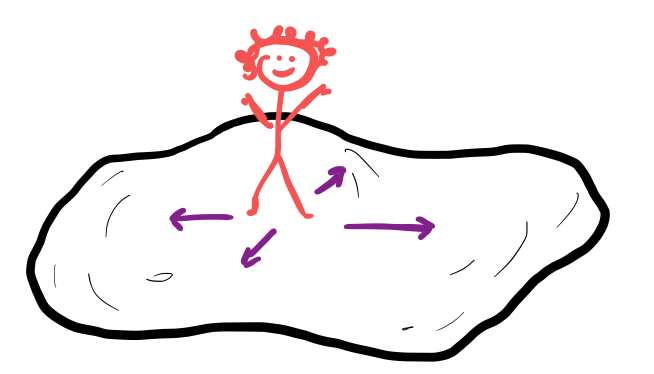
\includegraphics[width=5cm]{images/person_moving.png}\pause
  % You can move in two independent directions: forwards or backwards, and left or right. Let's pretend you're *really* small, so you don't notice that earth is uneven: to you, whereever you are, near you the surface of the earth looks like (part of) a disc.
  % TODO: slightly update the picture here!
  \raisebox{-8mm}{\makebox{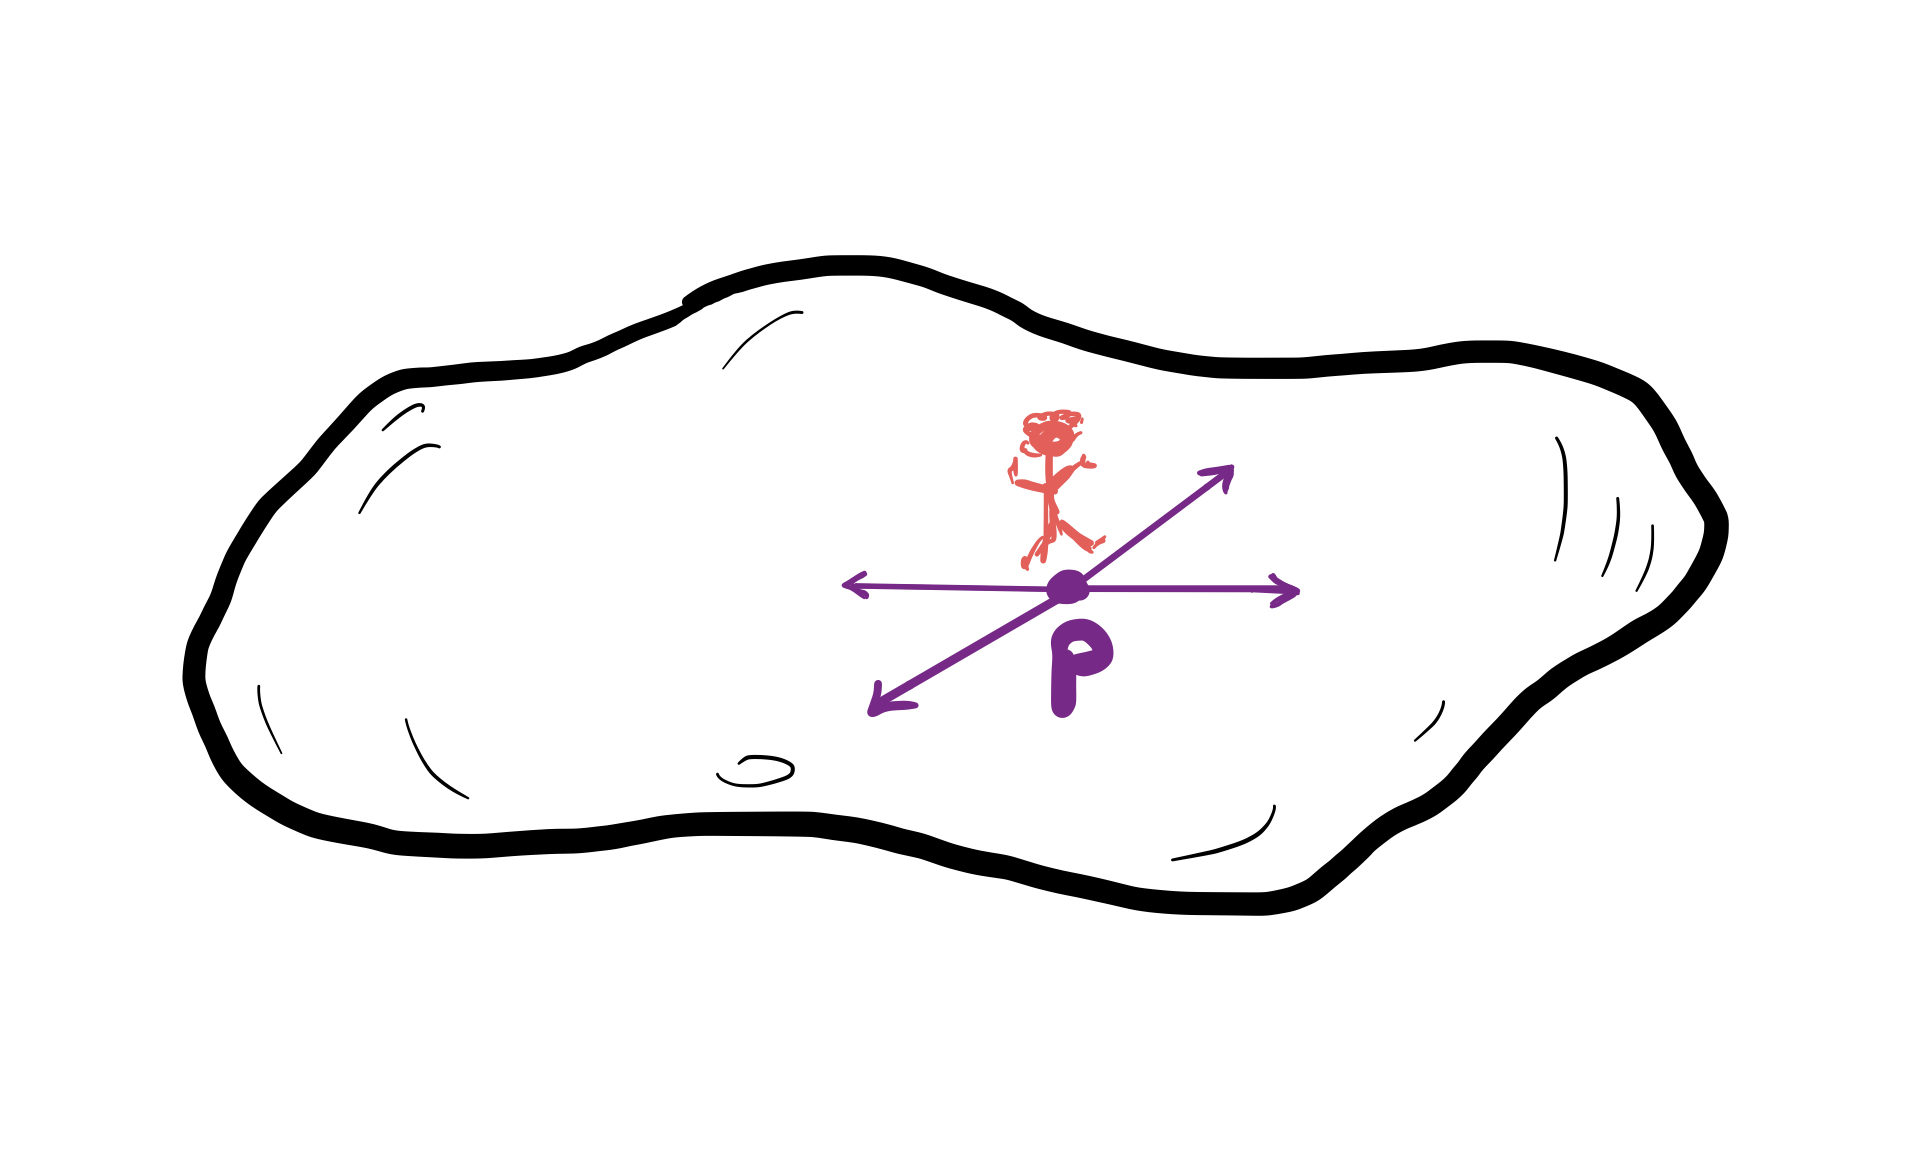
\includegraphics[width=6cm]{images/person_moving_directions.png}}}\\
  % In other words: earth' surface is an object which, locally looks, to an ant, like a part of a disk.
  earth is a manifold: locally looks like part of a disk
\end{frame}

\begin{frame}
  \frametitle{Smooth manifolds}
  % Let's generalise that to higher dimensions: an n-dimensional manifold M is a topological space which locally looks like R^n. We also call a two-dimensional manifold a surface.
  \begin{itemize}
    \item manifold: \shrink{second countable Hausdorff} topological space $M$ locally homeomorphic to $\R^n$

    % every point has an open nbhd homeomorphic to R^n (a coordinate chart); these charts overlap and transition functions are homeo
    \item every $p\in M$ has a coordinate chart:\\$p\in U\subset M$ open, homeomorphism $\phi\colon V\to U$ for $V\subset \R^n$
    % these charts form an open cover of $M$; the open cover of all charts is part of the datum of the manifold
    % whenever two charts overlap: there is a resulting coordinate transformation (which is a homeomorphism)
    % There are two technical details which I will not go into: we assume our space to be Hausdorff and second countable. Don't worry if you don't know what this means; basically all examples I would encounter in nature are these.

    % I'm a differential geometer, so all my manifolds today are smooth. This just means all transition maps between different charts are smooth.
    % One can have different smooth structures on the same topological manifold; we always talk about a manifold with a chosen smooth structure.
    % This is a restriction, but often not a big one. "Many" topological manifolds have a smooth structure; there are notably some manifolds which are not. (This is part of what Simon Donaldson got his fields medal for in 1986.)
    \item smooth manifold: all coordinate transformations from overlapping charts are smooth
    % I'll also sometime mention the boundary of a manifold: this is where a manifold looks like a half-space. For instance, the upper half of the plane is a manifold with boundary - the real axis.
    \item boundary: looks like upper half of $\R^n$
  \end{itemize}
  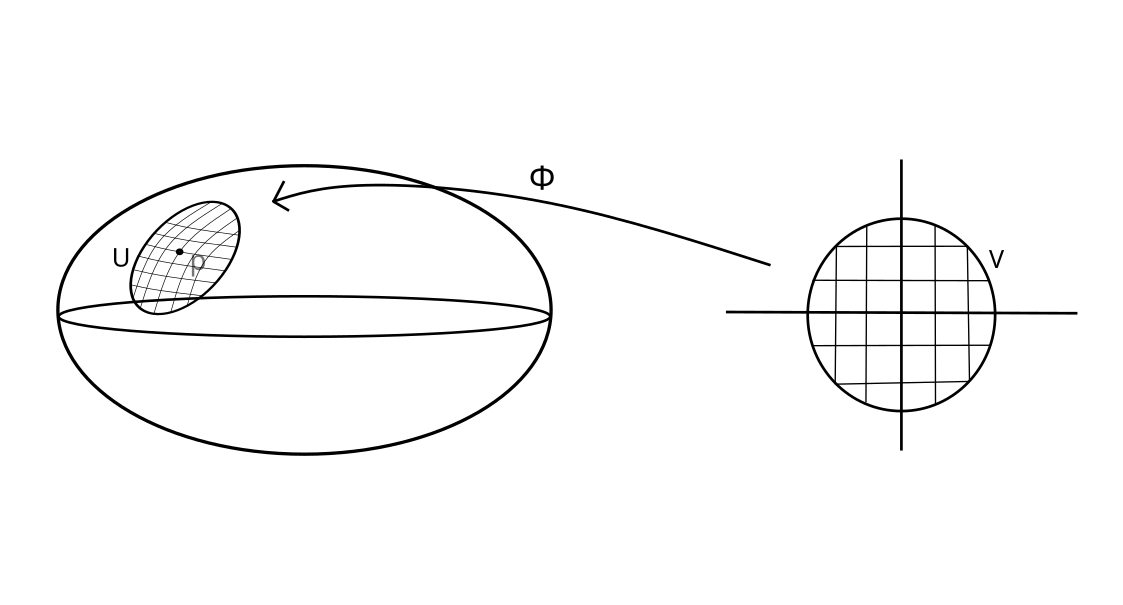
\includegraphics[width=8cm]{images/surface_with_chart.png}\\
  \tiny{Picture courtesy of Dominik Gutwein.}
\end{frame}

\begin{frame} % CAN SKIP
  \frametitle{Examples of smooth manifolds}
  % Let's look at some examples of manifolds. In general, taking the (disjoint) union of two n-manifolds yields another n-manifold - so we can focus on connected spaces.
  \begin{itemize}
  % A zero-dimensional manifold consists of isolated points, which is often not interesting.
  \item $n=0$: isolated points
  % In dimension 1, we can have a line, but also a circle.
  \item $n=1$: $\R$, $\sphere{1}$
  %\includegraphics[width=1cm]{images/line.png}
  %\includegraphics[width=1cm]{images/circle.png}
  % In dimension two, things get more interesting: the earth's surface is such an example. Topologically, it's homeomorphic to a sphere (or perhaps your favourite potato); we can also have a doughnut (or coffee cup) - but we could also take g tori and squish them together in a line (as drawn here). You'd call that a closed genus g surface. Of course, something like the real plane is totally fine as well.
  \item $n=2$: $\R^2$, $\sphere{2}$, $\T^2$, $\Sigma_g$ for $g\geq 1$\\
  \raisebox{4pt}{\mbox{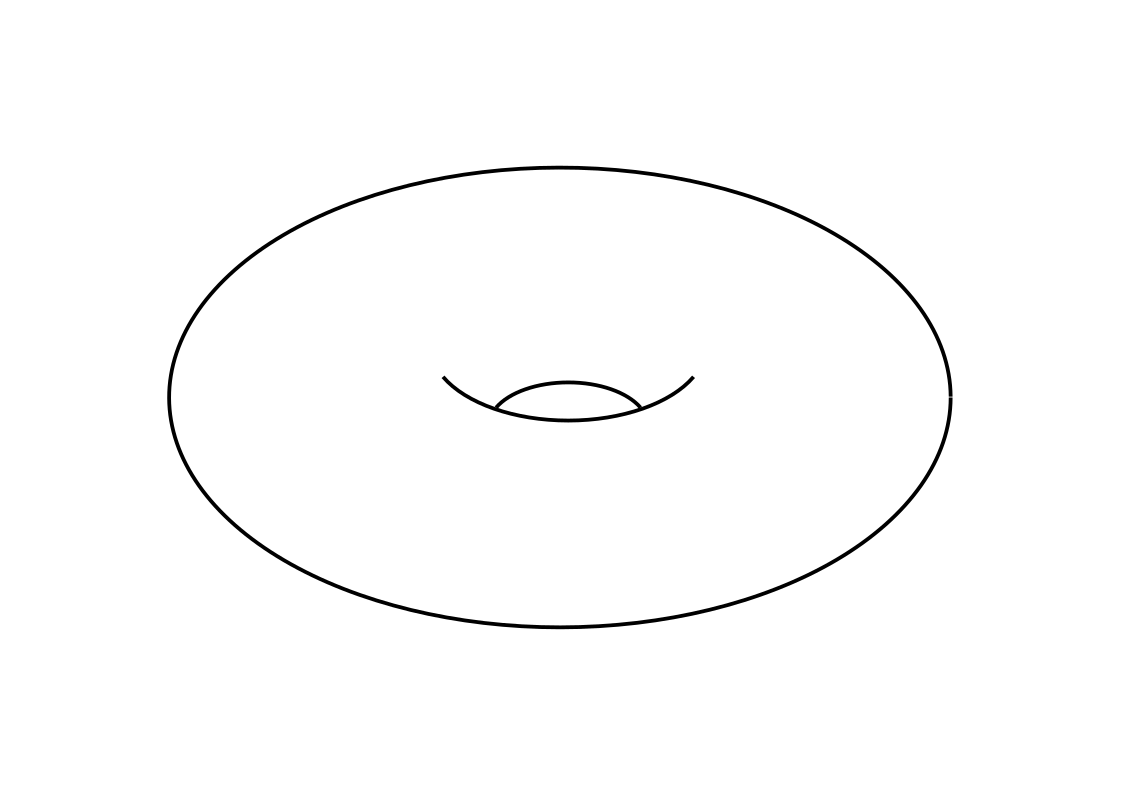
\includegraphics[width=1cm]{images/torus.png}}}
  
\includegraphics[width=1.5cm]{images/surface_genus_2.png}
  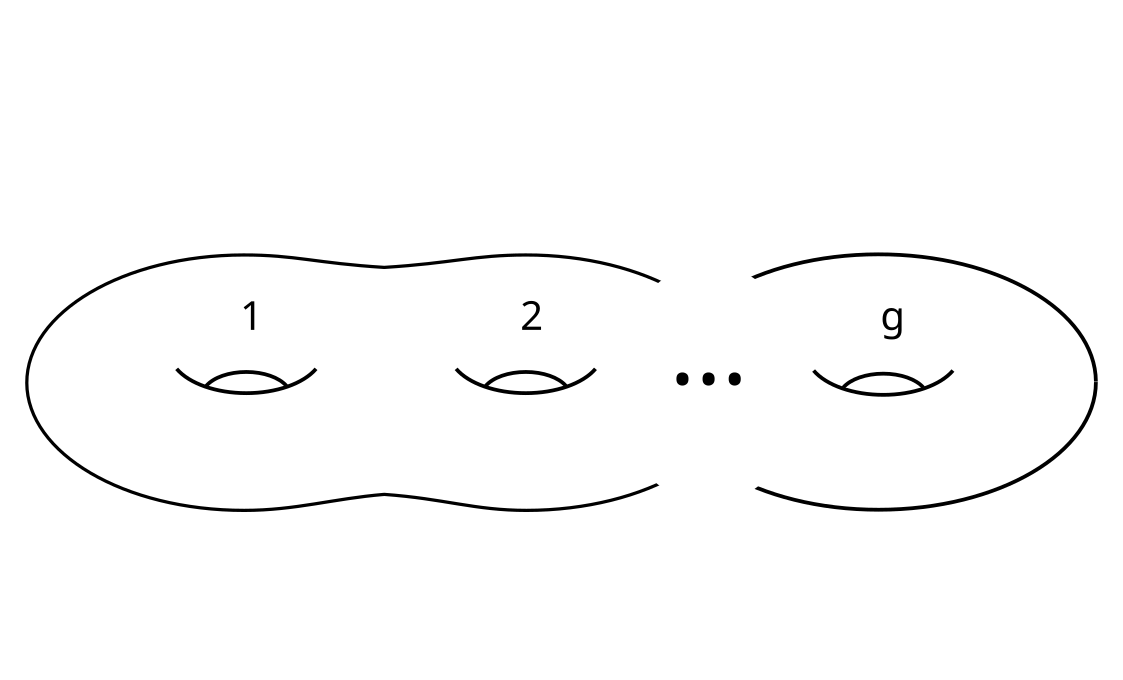
\includegraphics[width=2cm]{images/surface_genus_g.png}\pause
  % In higher dimensions, things get much more interesting and complicated. In dimension two, you have a list of all manifolds. You can still classify manifolds in 3 dimensions (but much harder); in four and higher dimensions, this is impossible.
  \item $n\geq 3$: complicated; classification for $n\geq 4$ impossible
  % For instance, in addition to spheres and tori, there are real and complex projective space. Algebraic geometers study smooth algebraic varieties (such as the Fermat quintic listed here).
  % One notable example are configuration space in physics and engineering: we'll see this again later.
  \item $n\geq 3$: $\R^n$, $\sphere{n}$, $\torus{n}$, $\RP{n}$, $\CP{n}$, $\{ [z_0\colon z_1\colon z_2\colon z_3\colon z_4]\in\CP{4}\;\mid\; z_0^5+\dots+z_4^5=0\}$\\
  configuration spaces in physics and engineering
  \end{itemize}
  % And some things which are not a manifold: the letter X is not a 1-dimensional manifold (at the crossing, it's not homeomorphic to a line segment)
\end{frame}

% Next, what is a symplectic manifold? To describe these, let's focus on dimension two first.
% How do you measure area in two dimensions? Given a small patch of a (smooth) surface, how shall we measure or define its area?
\begin{frame}
  \frametitle{How to measure area on a 2-manifold?}
  \begin{itemize}
  % For a subset of R^2, we obtain the area by integrating its characteristic function (w.r.t. a suitable measure).
  % If our patch is sufficiently small, we map it to R^2 via a chart and determine the area there: this amounts to integrating over a density function. Globally, we need to choose density functions in each chart in a compatible way: this amounts to a differential 2-form.
  \item locally: integrate density function
  \item globally: use a differential 2-form
  \end{itemize}
  \begin{columns}
    \begin{column}{0.7\textwidth}
      \begin{itemize}
        % To make this precise, we consider the *tangent space* at a point. Imagine the manifold placed inside some R^n (the Whitney embedding theorem tell us we can always do this). Geometrically, the tangent space at a point is the space of all vectors at this point which are tangent to a manifold. I'll skip a formal definition.
        % This is a real vector space, of the same dimension as the manifold. Moreover, a local chart induces a basis of the tangent space.
        \item each $p\in M$ has \highlight{tangent space} $T_pM$, $2$-dimensional $\R$-vector space
        % Now, a differential two-form locally specifies a density function for each local chart. Formally, it's a family of skew-symmetric bilinear maps on each tangent space, varying smoothly along the base point.
        \item $2$-form $\omega = \{\omega_p\colon T_pM\times T_pM\to \R\}_{p\in M}$\\ $\omega_p$ anti-symmetric bilinear,\\ smoothly varying with $p$
      \end{itemize}
    \end{column}
    \begin{column}{0.21\textwidth}
      % TODO use a better picture if I get one
      \vspace{3mm}\hspace{-8mm}\makebox{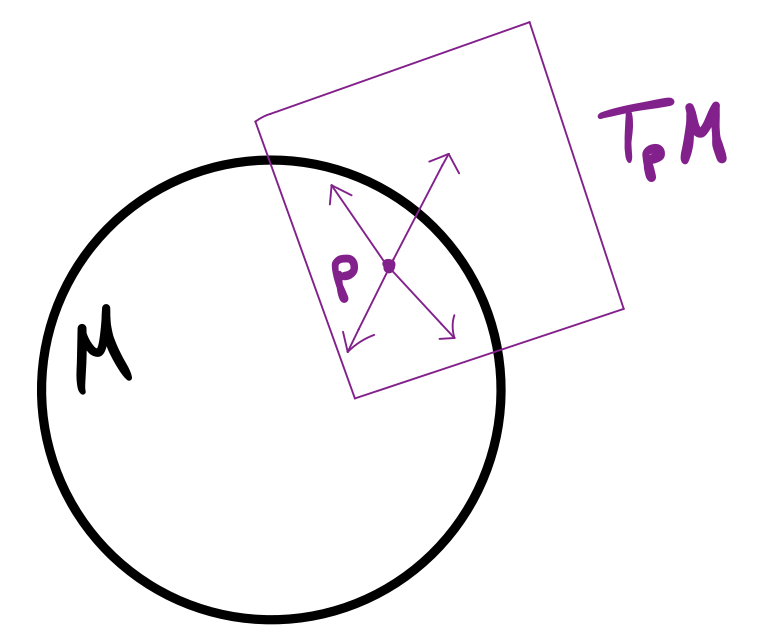
\includegraphics[width=3cm]{images/tangent_space_placeholder.png}}
    \end{column}
  \end{columns}
  \begin{itemize}
    % We call a 2-form an area form if each bilinear map is non-degenerate.
    \item \highlight{area form}: each $\omega_p$ is non-degenerate
    % A two-dimensional symplectic manifold is precisely a smooth surface with a choice of area form.
    \item \highlight{symplectic $2$-manifold}: $M$ plus choice of area form
  \end{itemize}
\end{frame}

\begin{frame}
  \frametitle{Symplectic manifolds}
  % In general, a symplectic structure on a smooth manifold is a choice of a non-degenerate closed 2-form. Non-degeneracy means each bilinear form is non-degenerate; closedness means its exterior derivative vanishes.
  \begin{definition}
    A symplectic manifold $(M,\omega)$ is a smooth manifold $M$ together with a closed non-degenerate $2$-form $\omega$.
  \end{definition}
  % For example, every orientable surface is a symplectic manifold: take any area form (which is automatically closed by dimension reasons).
  % Probably that definition wasn't very illuminating. Let's give a more geometric explanation. A symplectic structure assigns signed area of all (sufficiently local) closed curves.
  \begin{itemize}
    \item equivalently: atlas of charts $(x_1,y_1,\dots,x_n,y_n)$\\
    in which $\omega$ looks like $\omega_0=\sum_{i=1}^n dx^i\wedge dy^i$
    \item geometrically: symp.\ structure = signed area of closed curves
    % Consider an embedded closed curve in R²: it bounds a closed disc (by the Jordan curve theorem). Consider the area of this disc.
    \item for $\gamma$ embedded closed curve in $\R^2$ $\to$ $A(\gamma)$ signed area of enclosed disc
    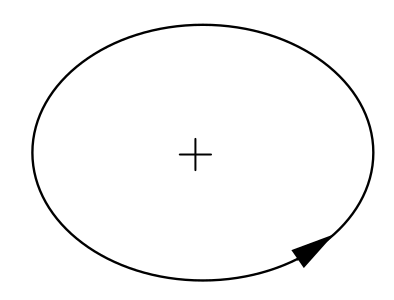
\includegraphics[width=2cm]{images/curve_orientation1.png}\pause
    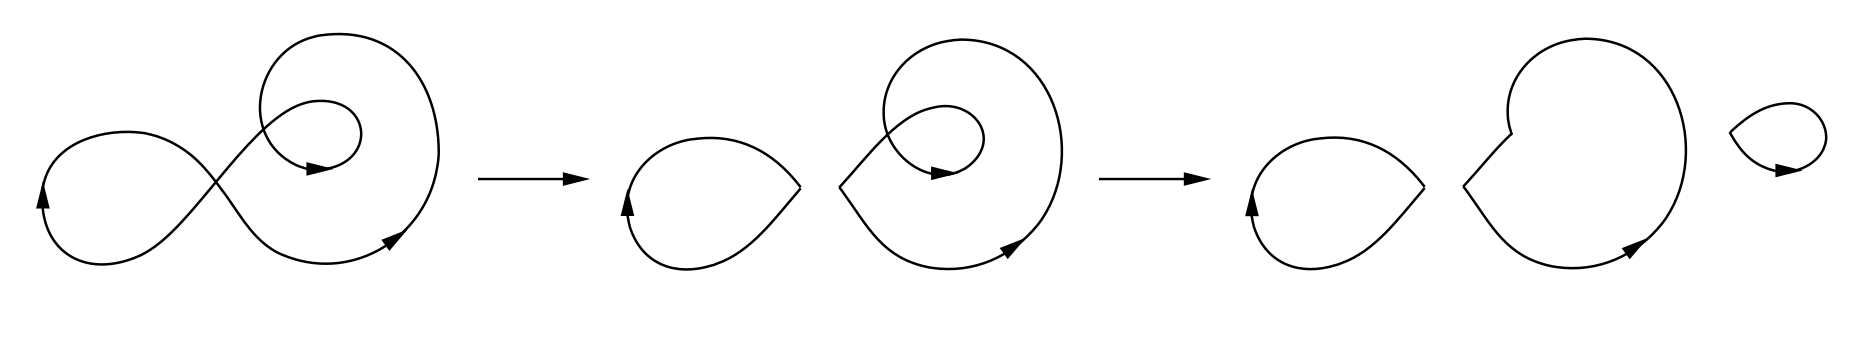
\includegraphics[width=7cm]{images/splitting_nonembedded_curve.png}
    \item $\gamma$ any oriented closed \shrink{piece-wise smooth} curve:\\ decompose into closed embedded pieces
  \end{itemize}
  \tiny{Pictures taken from Schlenk, \emph{Symplectic embedding problems old and new} (2017).}
\end{frame}

\begin{frame}
  \frametitle{Symplectic manifolds (cont.)}
  \begin{itemize}
    \item \highlight{standard symplectic structure} on $\R^{2n}$:\\
    map $\gamma\to A(\gamma)=A(\gamma_1)+\dots+A(\gamma_n)$,\\
    where $\gamma=(\gamma_1,\dots,\gamma_n)$ any closed oriented curve
    % Given a smooth manifold, choose an atlas: for any closed curve contained in a coordinate chart, we can determine its signed area.
    % A symplectic structure is a compatible way of making such choices.
    % In other words, it's an atlas whose transition functions preserve signed area.
    \item symplectic structure on $M$ is an atlas whose transition functions preserve signed area
    % why are these definitions the same? if \gamma bounds the disc D, Stokes shows A(\gamma)=\int_D \omega_std. Darboux' shows a symplectic structure is an atlas whose transition functions are symplectomorphisms.
    \hide{\item equivalence: Darboux' theorem and short computation}
  \end{itemize}
\end{frame}

\section{Motivation: Hamiltonian mechanics}

% Now we've seen what symplectic manifolds are. Why are these interesting?

\frame{
  \frametitle{Motivation: Hamiltonian mechanics}
  \pause
  \begin{minipage}{0.45\textwidth}
    \begin{figure}
      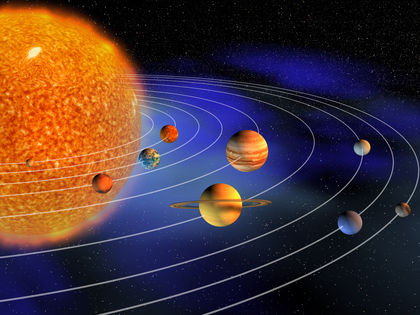
\includegraphics[width=5cm]{images/solar_system.jpg}\\
      The solar system (simplified).
%      \shrink{Source: \url{http://www.scienceclarified.com/photos/solar-system-2865.jpg}}
    \end{figure}
  \end{minipage}
  \hspace{1cm}
  \begin{minipage}{0.4\textwidth}
    \begin{figure}
      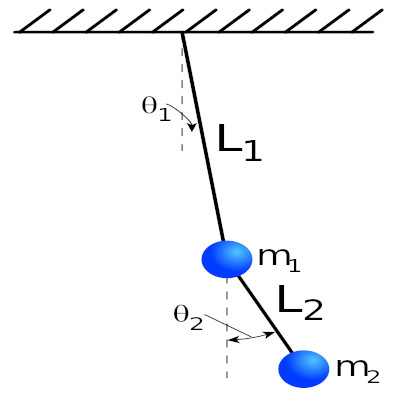
\includegraphics[height=3.5cm]{images/double_pendulum.jpg}\\
      A double pendulum.
%      \\\shrink{Source: By JabberWok, CC BY-SA 3.0, \url{https://commons.wikimedia.org/w/index.php?curid=1601029}}
    \end{figure}
  \end{minipage}
}
% One motivation comes from dynamical systems: there are many results about area-preserving maps in two dimensions (such as the Poincaré-Birkhoff theorem). In higher dimensions, there is a notion of volume-preserving maps, but the correct generalisation are symplectomorphisms. For instance, Poincaré-Birkhoff generalises into the Arnold conjecture. We'll see this again in a few moments.

% I'll tell you another reason, coming from classical physics.
% Consider a mechanical system. I've put two examples on my slide; the solar system and a double pendulum. They can be described by Newton's laws of mechanics, but perhaps slightly awkwardly: for instance, the pendulum's arm are rigid, this puts a constraint on the pendulum's evolution. We'd want our setup to encode such constraints. Hamiltonian mechanics is an equivalent way to describe Newton's axioms, but is more more elegant (and handles constraints nicely).

% So, let's dive in. Let's derive the correct framework in the example of the n-body problem (such as the solar system).
\begin{frame}
  \frametitle{Hamiltonian systems: from Newton's to Hamilton's equations}
  \begin{itemize}
    % for k particles moving in R^3, we have 3 degrees of freedom per particles, hence 3k degrees of freedom overall. generally, a
    \item system of particles moving with n degrees of freedom %is described by a path in $R^n$,
    \[ q(t) = (q_1(t),\dots q_n(t)) \]
    \item \hide{gravitational interaction is conservative:}
    forces are derived from a \highlight{potential} $V(q)$ by $F(q)= -\grad V(q)$
    \item Newton's second law states $m_i \ddot{q_j} = - \frac{\partial V}{\partial q_j}$
    \hide{\item total energy
      \[ E := \mymark{blue}{\sum_{j=1}^n \frac{1}{2} m_j\, \dot{q}_j^2}{kinetic energy} + \mymark{red}{V(q)}{potential energy} \]
      is conserved: $\frac{\partial E}{\partial t}=0$}
    \pause

    % The Irish physicist Hamilton realised a better viewpoint for this.
    % His idea was to consider the momenta of the particles.
    \item Hamilton: consider momenta $p_j := m_j \dot{q_j}$
    \item total energy defines the Hamiltonian function
    \[ H\colon \R^{2n}\to\R,\quad (q,p)\mapsto \mymark{red}{\sum_{j=1}^n \frac{p_j^2}{2 m_j}}{kinetic energy} + \mymark{blue}{V(q)}{potential forces} \]
    \vspace{-\baselineskip}
    \item Newton's equations become \highlight{Hamilton's equations}
    \begin{equation*} \dot{q}_j = \frac{\partial H}{\partial p_j} \;\;\text{ and }\;\,\dot{p}_j = -\frac{\partial H}{\partial q_j}, \quad \text{ for }j=1,\dots n \tag{H}\end{equation*}
  \end{itemize}
\end{frame}

\begin{frame}
  \frametitle{Hamilton's equations on a manifold: symplectic manifolds}
  \begin{columns}
    \begin{column}{0.72\textwidth}
      \begin{itemize}
        % Hamilton's key insight was to treat the positions $q_j$ and momenta $p_j$ as independent variables, and to describe the motion of the system as a trajectory in $2n$-dimensional ``phase space''.
        \item key insight: regard $(q(t), p(t))$ as trajectory\\in \highlight{phase space} $\R^{2n} = T^\ast \R^n$

        % This is useful, since the phase space formalism also applies to the double pendulum! If we assume that both pendulums are rigid, we can describe the double pendulum by the two angles only, hence by two coordinates $q(t)=(q_1(t), q_2(t))$ in the torus. The phase phase turns out to be the cotangent bundle of the position space.
        \item double pendulum: rigid arms \hide{and no friction} mean\\
        $q(t)=(q_1(t),q_2(t))\in \torus{2}$,\\phase space is cotangent bundle $T^\ast \torus{2}$
        % you may observe that \R^{2n}$ is the phase space of the position space \R^n above; this observation holds in general

        \item for systems with constraints, treat $(q,p)$\\as \highlight{local coordinates} of a point\\moving in a manifold
      \end{itemize}
    \end{column}
    \begin{column}{0.3\textwidth}
      \hspace{-8mm}\mbox{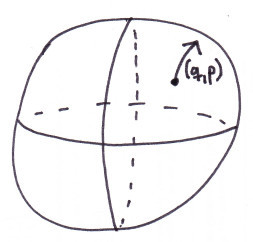
\includegraphics[width=4cm]{images/phase_space.jpg}}
    \end{column}
  \end{columns}

  \vspace{0.5\baselineskip}
  % issue: a system which satisfies Hamilton's equations for one choice of local coordinates need not satisfy it for all other choices. This motivates the following definition.
  \begin{block}{Fact}
    A smooth $2n$-dimensional manifold it is covered by coordinate charts $(q_1, p_1,\dots, q_n, p_n)$ such that for all smooth $H\colon M\to\R$, all coordinate changes preserve the form of (H) iff it is symplectic.
  \end{block}
  % Both R^2n and the cotangent bundle of any smooth manifold are symplectic.
\end{frame}

\begin{frame}
  \frametitle{Hamilton's equation in symplectic manifolds}
  \begin{definition}
    For $(M, \omega)$ symplectic, $H\colon \R\times M\to\R$ smooth, the \highlight{Hamiltonian vector field} $X_{H_t}$ of $H$ is defined by $\omega(X_{H_t}, \cdot) = -dH(t,\cdot)$.
    % an equality of $1$-forms; non-deg. of $\omega$ implies that $X_H$ is uniquely defined.
  \end{definition}
  \begin{block}{Exercise}
    Solutions $(q,p)$ of (H) are the integral curves of $X_H$.
    %A path $x(t)=(q(t),p(t))$ in $\R^{2n}$ satisfies Hamilton's equation iff $\dot{x}(t) = X_H(x(t))$. Thus: trajectories of a Hamiltonian system are integral curves = flow lines of the Hamiltonian vector field $X_H$!
  \end{block}
  % To summarize: symplectic manifolds are the natural setting for describing the evolution of Hamiltonian systems.
\end{frame}

\section{Some sample results}

% I've told you a lot *about* symplectic geometry by now; let's dive in and see some open or solved problems. Two theorems are related to Hamiltonian dynamics: what can we say about periodic Hamiltonian orbit?
\begin{frame}
  \frametitle{Sample theorems I: fixed points of dynamical systems}
  % I'll skip the definition of non-degeneracy and just note that almost any Hamiltonian is non-degenerate. If you pick one at random, it's non-degenerate.
  \begin{block}{Arnold conjecture}
    If $M$ is a closed* symplectic manifold and $H\colon\sphere{1}\times M\to \R$ smooth and non-degenerate, then
    \vspace{-0.5\baselineskip}
    \[ \#\; \text{$1$-periodic orbits of $X_H$} \geq \sum_{i=1}^n b_i(M),\]
    where $b_i(M) := \rk{H_i(M)}$ is the $i$-th Betti number of $M$.
  \end{block}
  % "mostly" solved: groundwork by Conley-Zehnder and Andreas Floer
  % under certain technical assumptions (removal tricky!); proposed solutions, but no consensus on the details yet

% TODO: this is wrong! need to explain Hamiltonian diffeo...
  \begin{block}{Conley conjecture}
    If $M$ is a closed symplectic manifold with e.g.\ $\pi_2(M)=0$ and $H\colon \sphere{1}\times M\to\R$ is smooth and non-degenerate,
    $X_H$ has infinitely many \shrink{simple} orbits of integer period.
    % includes torus! and all symplectically aspherical ones.
    % Ginzburg-Gürel's survey contains recent results
  \end{block}
\end{frame}

% I have another application area for you, related to symplectic fillings. What is that?
\begin{frame}
  \frametitle{Sample theorems II: symplectic fillings}
  \begin{definition}
    A \highlight{smooth filling} of a smooth manifold $M$ is a compact manifold $N$ with $\boundary N\cong M$.
    % necessarily, $N$ has dimension one larger than $M$
  \end{definition}
  % Not every smooth manifold has a smooth filling: for example, complex projective space is not the boundary of any 5-manifold. However, this question is well-understood by now (and is solved by bordism theory).
  not always possible ($\CP{2}$ has no smooth filling),\\but understood (bordism theory, 1960s)\pause
  % So let's make the problem more interesting and consider this symplectically. The boundary of a symplectic manifold is odd-dimensional, hence cannot be symplectic any more --- but carries the odd-dimensional analogue of a symplectic structure, called a contact structure.
  % A contact manifold is an odd-dimensional smooth manifold together with a contact structure: choosing a 1-form s.t. ... and taking its kernel at each point. (So, a contact structure is a collection of hyperplanes.)
  \begin{definition}
    A \highlight{contact manifold} $(M^{2n-1},\xi=\ker\alpha)$ is a smooth manifold $M$ together with a choice of $1$-form $\alpha$ s.t.\ $\alpha\wedge d\alpha^{n-1}\neq 0$.
  \end{definition}
  % So, the definition we're interested in is the following. Let's call this a template definition because there are various kinds of symplectic fillings. (This matters: a manifold can be fillable in one sense but not the other.)
\begin{block}{Template definition}
  A \highlight{symplectic filling} of $(M,\xi)$ is a compact symplectic manifold $(W,\omega)$ with $\boundary W\cong (M,\xi)$. % and orientations match
\end{block}
\end{frame}

\begin{frame}
  \frametitle{Sample theorem II: symplectic fillings (cont.)}
  \begin{block}{Template definition}
    \fade{A symplectic filling of $(M,\xi)$ is a compact symplectic manifold $(W,\omega)$ with $\boundary W\cong (M,\xi)$.}
  \end{block}
  % Today, I'll only mention exact fillings, which are the following.
  \begin{definition}
    An \highlight{exact symplectic filling} of $(M,\xi)$ is a compact symplectic manifold $(W,\omega=d\lambda)$ s.t.\ $\boundary W\cong (M,\xi)$ and the vector field $X$ induced by $\iota_X \omega=\lambda$ points outwards along $\boundary W$.
  \end{definition}

  \begin{theorem}[Zhou '20,'22]
    If $n\geq 3$ and $n\neq 4$, $(\RP{2n-1}, \xi_\std)$ has no exact symplectic filling.
  \end{theorem}
\end{frame}
% This list is by no means exhaustive. For instance, I've skipped Gromov's non-squeezing theorem and symplectic capacities, as Shah will talk about them tomorrow.

\begin{frame}
  \frametitle{Underlying paradigm: symplectic invariants}
  \begin{itemize}
    % Let's look at the machinery behind these sample theorems. As different as they look and are, their proofs share a common feature: they are related to invariants of symplectic manifolds.
    % For instance, the Arnold and Conley conjecture use an invariant called Hamiltonian Floer homology.
    \item Arnold, Conley conjecture: use \shrink{Hamiltonian} Floer homology

    % Given a closed symplectic manifold, choose a non-degenerate Hamiltonian and consider the $1$-periodic Hamiltonian orbits. Hamiltonian Floer homology of $M$ is generated by these orbits. More precisely, it's the homology of a chain complex defined by these orbits. Hence, the rank of the homology gives a lower bound on the number of orbits. Relating the Betti numbers to the rank of Hamiltonian Floer homology completes the proof.
    \item $(M,\omega)$ symplectic $\to$ homology groups $HF_\ast(M)$,\\ generated by $1$-periodic Ham.\ orbits $\mathcal{P}(H)$
    \item Arnold conjecture: bound \# orbits via $\rk HF_*(M)$

    % For the Conley conjecture, we pass to k-periodic orbits of $H_t$. The actual analysis is more involved.
    \item Conley conjecture: pass to higher iterates
    % the third theorem (about symplectic fillings) uses another invariant called (positive) symplectic homology; will skip for now (ask me at the end if you want me to explain more)
    \item Zhou's theorem: use (action-filtered) positive symplectic homology of hypothetical filling
  \end{itemize}
\end{frame}

\begin{frame}
  \frametitle{Details: Hamiltonian Floer homology}
  given: $(M,\omega)$ closed* symplectic manifold; $H\colon \sphere{1}\times M\to \R$ smooth, non-degenerate% e.g. symplectically aspherical
  \begin{itemize}
    \item \highlight{Floer chain complex} $(CF_*(M,\omega),\partial)$
    \item Hamiltonian Floer homology $HF(M,\omega)=H_*(CF_*(M,\omega)))$
    \item $CF_*(M)$ generated by $1$-periodic orbits of $X_H$
    \item \shrink{\fade{grading by Conley-Zehnder index}}
    % differential: contribution of one orbit to the other is given by counting Floer cylinders asymptotic to these orbits
    \item differential counts \shrink{finite energy} \highlight{Floer cylinders}\\connecting two $1$-periodic orbits
    % one can show that this is well-defined (that we indeed get a chain complex and that there are always finitely many cylinders); one can also show independence of the choice of Hamiltonian
    \item show: well-defined; independent of $H$
    % I will not get into details of this, but instead focus on holomorphic curve - Floer cylinder can be seen as a special case of them
  \end{itemize}
\end{frame}

\section{Pseudo-holomorphic curves}
% We have now entered the machine room of our proof and seen some ingredients in motion. Let's examine our main machine in more detail. I've promised you pseudo-holomorphic curves, so here we go. What is a pseudo-holomorphic curve?
% Hearing "holomorphic", we'd expect something whose differential is complex linear, so we should talk about what complex multiplication means.
\begin{frame}
  \frametitle{Pseudo-holomorphic curves}
  \begin{definition}
    An \highlight{almost complex structure} on a smooth manifold $M$ is a collection of maps $J_p\colon T_pM\to T_pM$ with $J_p^2=-\id$, smoothly varying in $p$.
  \end{definition}
  % morally, an almost complex structure corresponds to multiplication by i on each tangent space (and indeed, each tangent space becomes a complex vector space this way)
  \begin{theorem}
    Every symplectic manifold admits an almost complex structure.
  \end{theorem}
  % In fact, there are many possible choices of almost complex structure. You should regard the choice of acs as an auxiliary object; the particular choice is not important. For instance, the space of all compatible acs is contractible - which implies many constructions are independent of the *choice* of acs.
\end{frame}

\begin{frame}
  \frametitle{Pseudo-holomorphic curves}
    % An almost complex manifold is a smooth manifold with a choice of almost complex structure. A pseudo-holomorphic curve is a map between two almost complex manifolds - that explains the word "ps-holo". It's domain is one-dimensional; we already saw them today.
  \begin{definition}
    A \highlight{Riemann surface} is a smooth surface with a choice of almost complex structure.
  \end{definition}
  % Today, we are interested in closed Riemann surfaces: compact without boundary. In fact, we have already seen all of them. If Sigma is a Riemann surface, it is diffeomorphic (and even biholomorphic) to the standard genus g surface, for some g\geq 0. We call g the genus of $\Sigma$
  % One can talk about punctured Riemann surfaces (not today; Floer cylinders are punctured holo curve). I don't think surfaces of infinite type are ever studied...
  \begin{fact}
    If $(\Sigma,j)$ is a Riemann surface and $\Sigma$ is closed, then $(\Sigma,j)\cong (\Sigma_g,j')$ for some $g\geq 0$. We call $g$ the \highlight{genus} of $\Sigma$.
  \end{fact}
  \begin{definition}
    A \shrink{closed} \highlight{pseudo-holomorphic curve} is a smooth map $u\colon (\Sigma,j)\to (M,J)$ with $J\circ du=du\circ j$,
    where $(\Sigma,j)$ is a closed Riemann surface and $(M,J)$ an almost complex manifold.
  \end{definition}
  % In case you get confused: a pseudo-holomorphic curve is (the image of)a two-dimensional real manifold --- but as a complex manifold, it's one-dimensional (hence called a curve).
\end{frame}

\begin{frame}
  \frametitle{Moduli space of holomorphic curves}
  % one key idea is to consider the moduli space of all holomorphic curves with given data
  % We've already seen that we can group them by their genus. We can also group by their homology class, the pushforward of the domain's fundamental class under the curve

  given: $(M,\omega)$ symplectic, almost complex structure $J$ on $M$\\
  for $g\geq 0$ and $A\in H_2(M)$, consider the \highlight{moduli space} of holomorphic curves
  \[ \mathcal{M}_g(A,J) := \{ u\colon (\Sigma,j)\to (M,J)\;\mid\; \text{u ps.-holo}; \Sigma\cong\Sigma_g, u_*[\Sigma]=A \}/_\sim \]
  % we quotient by reparametrisation (i.e. relating by a biholomorphic map on Sigma): fundamentally, in applications we care about the image of the curve in M

  intuition: $J$ is an auxiliary object
  % In our dream world, every moduli space is a compact smooth manifold. In fact, there is a formula for its dimension in terms of A and g.
  \begin{block}{Wishful thinking}
    $\mathcal{M}_g(A,J)$ is a compact smooth manifold (and finite-dimensional).
  \end{block}
\end{frame}

\begin{frame}
  \frametitle{Understanding the moduli space of holomorphic curves}
  \begin{block}{Wishful thinking}
    \fade{$\mathcal{M}_g(A,J)$ is a compact smooth manifold (and finite-dimensional).}
  \end{block}
  % How would we approach proving this? We can use the implicit function theorem. Let's rephrase the equation defining a holomorphic curve: multiply both sides by J and use J²=-id.
  \begin{itemize}
    \item rephrase: $u\colon (\Sigma,j)\to (M,J)$ is $J$-holomorphic iff $J\circ du\circ j=-du$ iff $du+J\circ du\circ j=0$
    % in other words, the moduli space is the zero set of the map sending u and J to du plus J composed with du composed with j
    \item so: $\mathcal{M}_g(A,J)$ is the zero set of $\Phi\colon(u,J)\mapsto du+J\circ du\circ j$
  \end{itemize}
  \pause
  % This is the kind of statement coming from the implicit function theorem.
  \begin{block}{\shrink{Finite-dimensional} Implicit function theorem}
    $E\to B$ smooth vector bundle, $s\colon B\to E$ smooth section transverse to the zero section. Then $s^{-1}(0)\subset B$ is a smooth submanifold.
  \end{block}
  % Looking closely: the map above lives in a vector bundle --- its base is the product of all smooth maps from Sigma to M with the space of all acs. This is infinite-dimensional (as is its rank).
  domain of $\Phi$ is $C^\infty(\Sigma,M)\times\mathcal{J}(M,\omega)$,
  where $\mathcal{J}(M,\omega)$ is the space of all \shrink{compatible} almost complex structures
\end{frame}

% The implicit function also holds in infinite dimensions, but with extra hypotheses. This adds further complications.
\begin{frame}
  \frametitle{Infinite-dimensional complications}
  \fade{$\mathcal{M}_g(A,J)$ is the zero set of $\Phi\colon C^\infty(\Sigma,M)\times\mathcal{J}(M,\omega)\to \dots$, $(u,J)\mapsto du+J\circ du\circ j$}
  \begin{itemize}
    % One additional condition in infinite dimensionals issue is that the linearisation of the section has a bounded right inverse. (This is automatic in finite dimensions.) This follows as the linearisation of Phi will be a Fredholm operator.
    \item linearisation of section has a bounded inverse:\\ok, $d\Phi$ is a \highlight{Fredholm operator}\pause

    % perhaps the biggest one: the domain of a Phi is not complete; the space of smooth maps is not complete - hence we cannot apply the IFT
    \item domain must be a \highlight{Banach manifold}:\\
    but $C^\infty(\Sigma,M)$ is not complete!
    % The solution is to extend Phi to a larger domain which is complete. Most commonly, we extend to a suitable Sobolev space of maps.
    % The condition $kp>2$ is necessary so the Sobolev embedding theorem guarantees continuity of our Sobolev maps.
    \item solution: extend $\Phi$ to a larger domain,\\
    e.g.\ \highlight{Sobolev spaces} $W^{k,p}(\Sigma,M)$ for $kp>2$
    % A priori, the zero set of this extended Phi could be larger: in our case, we can exclude this. The Cauchy-Riemann equation is an elliptic partial differential equation. Hence we can apply regularity results for elliptic operators to show that every solution of the C-R eqn is in fact smooth.
    \item \highlight{elliptic regularity}: extension has same zero set
  \end{itemize}
  % Note two things I have not talked about: transversality of the section and compactness of the moduli space. That comes now.
\end{frame}

\begin{frame}
  \frametitle{Bad news: transversality and compactness}
  % Our wishful thinking was too optimistic for two further reasons.
  \begin{itemize}
    % firstly, the moduli space is not compact: but it can be compactified. We just need to add some condition on our almost compatible structure. For instance, it suffices to assume the the acs is compatible, i.e. plugging it into the symplectic form induces a Riemannian metric.
    \item $\mathcal{M}_g(A,J)$ is not compact, but compactifiable:\\
    require compatible $J$ (i.e. $\omega(\cdot,J\cdot)$ Riemannian metric)
    % secondly, transversality is not always true: there are examples of J such that M is not a manifold. The best we can hope for is that almost any J satifies this. (For the experts: the set of such J is comeagre.)
    \item transversality failure: for some $J$, $\mathcal{M}_g(A,J)$ is not a manifold\\
    best case: holds for ``generic'' $J$
    % In fact, even that is too much to ask: as a rule of thumb, transversality results are incompatible with symmetries.
    % One instance of this are multiply covered curves: a holomorphic curve is multiply covered iff it factors through a (possibly branched) cover of Riemann surfaces. The cover's deck transformations act on the curve, obstructing transversality.
    % (Of course, this also applie if an external group acts on M.)
    \item more generally: transversality doesn't like symmetry\\
    e.g. multiply covered curves (or external group action)
  \end{itemize}
% To summarise: the space of all simple curves (not multiply covered) is a smooth manifold, for generic compatible $J$.
\begin{theorem}
  For ``almost all'' compatible $J$, $\mathcal{M}^*_g(A,J)$ is a smooth compactifiable manifold\shrink{ of dimension $(n-3)(2-2g)+2\langle c_1(TM), A\rangle$}.
\end{theorem}
\end{frame}

\section*{Summary}
% To conclude: we have seen what symplectic manifolds are; describing the evolution of a mechanical system naturally leads to a symplectic manifolds.
% Symplectic geometry can answer questions about periodic orbits of these mechanical system: by defining invariants based on counting pseudo-holomorphic curves.
% Defining and understanding them requires understanding moduli spaces of holomorphic curves, with significant technical machinery.
\begin{frame}
  \frametitle{Summary}
  \begin{enumerate}
    \item Symplectic manifolds arise when describing mechanical systems.
    \item Periodic orbits of Hamiltonian systems can be understood using symplectic invariants.
    \item These invariants are defined using moduli spaces of pseudo-holomorphic curves.
  \end{enumerate}
  \pause
  \vspace{2\baselineskip}{\LARGE Thanks for listening! Any questions?}
\end{frame}

\end{document}
